\section{Aluminiumoxid-ALD}
\label{aluminaald}

Einen beispielhaften Prozess für Atomlagenabscheidungen bildet die Abscheidung von Aluminiumoxid \ce{Al2O3}\cite{puurunen_surface_2005}, für die häufig das Precursorpaar Trimethylaluminium (TMA, \ce{Al(CH4)3}) und Wasser genutzt wird.
Mit einer Permittivität von $k=\approx 8$ hat Aluminiumoxid neben anderen Materialien das zuvor geläufige Siliziumdioxid ($k=3.9$) in der Halbleiterindustrie etwa in modernen Prozessoren ersetzt, obwohl die Reaktionsmechanismen nicht vollends verstanden sind\todo{dringend ref!}.
Deshalb soll der TMA-\ce{H2O}-Prozess im Folgenden besonders hinsichtlich der Reaktion der Precursormoleküle mit der Oberfläche untersucht werden.
Einige Reaktionen des Wasser-Halbzyklus' wurden erfolgreich simuliert, wo hingegen die Simulation des TMA-Halbzyklus' bisher nicht erfolgreich war.

\subsection{Parametersätze}

Die Zahl der verfügbaren Parametrisierungen reduziert sich für \ce{Al2O3} auf drei Kandidaten, die bereits aus den Untersuchungen der Silizium-Potentiale bekannt sind:\\
\todo{Stil ok?}\texttt{Al\_AlO\_AlN}, \texttt{liu\_ettringite}, das nachfolgend nur unter der Bezeichnung \texttt{liu} geführt werden soll, und \texttt{narayanan}.

Die Al\_AlO\_AlN-Datei stammt direkt aus der offiziellen LAMMPS-Distribution, wurde jedoch spätestens in der Version vom 17. Dezember 2014 aus dem Paket genommen, was vermutlich durch die schlechte Darstellung der Materialeigenschaften von Bulk-Materialien liegt, wie nachfolgend untersucht wird.

Bei der Liu-Potentialdatei rührt die Unterstützung für sowohl Aluminium als auch Silizium von der Abwandlung einer bestehender Parametrisierungen, die bereits Silizium unterstützt hat.
Da jedoch bei der Erweiterung auf Ettringit (\ce{Ca6[Al(OH)6]2(SO4)3 26H2O}) die Konsistenz der Silizium-Parameter nicht bewahrt wurde, können Silizium-Materialien damit nicht verlässlich simuliert werden, wie in Abschnitt \ref{siliconpvd} gezeigt wurde.
Ettringit hingegen enthält \ce{Al}-\ce{O}-Bindungen und \ce{OH}-Gruppen, so dass zumindest die Simulation des Bulkmateriales und einer hydroxylierten Oberfläche aussichtsreich erscheint.

Die Narayanan-Parametrisierung lässt aufgrund ihrer Herkunft als Potential für \ce{Li-Al}-Silikate für die Simulation von Eukryptit (\ce{LiAl[SiO4]}) endgültige Aussage über die Qualität der \ce{Al}-\ce{O}-Bindungen und \ce{OH}-Gruppen zu.
Zwar besteht der Trainingssatz aus Lithium-Aluminium-Kristallen, aber nur $\gamma$-\ce{LiAlO2} beinhaltet direkte \ce{Al}-\ce{O}-Bindungen, während keine der für das Fitting genutzten Strukturen Wasserstoff beinhaltet.
Es ist daher unwahrscheinlich, dass die Narayanan-Potentialdatei komplizierte Systeme verlässlich darstellt.

\subsection{Untersuchungen}

Anders als in den vorherigen Abschnitten dieses Kapitels wird keine vollständige Parsivald-Simulation durchgeführt, sondern stellen die Voruntersuchungen die eigentlichen Untersuchungen des Kapitels dar, in denen neben Eigenschaften des Bulkmateriales auch Precursormoleküle und deren Reaktion mit der Oberfläche simuliert werden.

\subsubsection{Bulkeigenschaften}

Zum Vergleich der strukturellen Eigenschaften des Bulkmateriales, wie etwa Dichte, Bindungslänge und Koordinationszahlen, wurde eine $\alpha$-\ce{Al2O3}-Struktur bei \SI{1500}{\kelvin} relaxiert.
Der eigentliche Referenzwert der Dichte bei Raumtemperatur liegt bei \SI{3.9}{\gpcc}, jedoch wurden die Strukturen durch einen methodischen Fehler nicht ausreichend relaxiert, weshalb er anhand der Relaxationstemperatur korrigiert werden muss.
Damit ergibt sich ein korrigierter Referenzwert zwischen \SI{3.95}{\gpcc} bei \SI{300}{\kelvin} und \SI{3.8}{\gpcc} bei \SI{1500}{\kelvin}\cite{fiquet_temperature_1999}, der im direkten Vergleich als \SI{3.85}{\gpcc} angenommen wird.

Zur Bestimmung der Dichte der amorphen Struktur wurde das Bulkmaterial über den Schmelzpunkt von \SI{2317}{\kelvin} auf \SI{2555}{\kelvin} erhitzt, auf dieser Temperatur relaxiert und langsam auf Raumtemperatur abgekühlt.
Aufgrund der strukturellen Unterschiede bei amorphen Aluminiumoxiden lässt sich keine eindeutige Referenzdichte angeben, so dass auf den Wertebereich von \SIrange{3.2}{3.6}{\gpcc} zurück gegriffen werden muss.

Bindungslängen und Koordinationszahlen wurden direkt aus der radialen Verteilungsfunktion bestimmt, wobei die Referenzwerte auf gleiche Weise durch die Untersuchung der Ausgangsstruktur bestimmt wurden, welche mittels Materials Studio auf Basis eines $\alpha$-\ce{Al2O3}-Kristalles präpariert wurde.

\begin{table}
  \caption[Vergleich struktureller Eigenschaften von Bulk-\ce{Al2O3} mit verschiedenen Parametersätzen]{
    Vergleich struktureller Eigenschaften von Bulk-\ce{Al2O3} mit verschiedenen Parametersätzen.
    Bindungslängen und Koordinationszahlen stammen von einer relaxierten Kristallstruktur.
  }
  \label{tab:aluminabulks}

  \begin{tabularx}{\textwidth}{|Xllll|}
    \hline
    \textbf{Eigenschaft}         & \textbf{Referenz}    & \textbf{Al\_AlO\_AlN} & \textbf{liu}         & \textbf{narayanan}   \\
    \hline
    Dichte, amorph               & \SI{>3.2}{\gpcc}     & ~                     & \SI{3.66}{\gpcc}     & ~                    \\ 
    Dichte, kristallin           & \SI{3.85}{\gpcc}     & \SI{4.31}{\gpcc}      & \SI{3.88}{\gpcc}     & \SI{3.76}{\gpcc}     \\
    \ce{Al}-\ce{O}-Bindungslänge & \SI{1.90}{\angstrom} & \SI{1.94}{\angstrom}  & \SI{1.88}{\angstrom} & \SI{1.85}{\angstrom} \\
    \ce{Al}-\ce{O}-Koordination  & \num{4.00}           & \num{5.40}            & \num{4.55}           & \num{4.05}           \\
    \ce{Al}-\ce{Al}-Koordination & \num{4.00}           & \num{6.66}            & \num{5.98}           & \num{5.10}           \\
    \ce{O}-\ce{O}-Koordination   & \num{12.0}           & \num{12.4}            & \num{11.0}           & \num{12.2}           \\
    \hline
  \end{tabularx}
\end{table}

Die Ergebnisse dieser Untersuchungen (Tabelle \ref{tab:aluminabulks}) zeichnen ein vielseitiges Bild.
Einerseits stimmen die Bindungslängen für alle Parametrisierungen auf \SI{2}{\percent} überein, andererseits ergeben sich aber große Unterschiede in der Dichte der Kristalle, die nicht über die Bindungslängen erklärbar sind.

So liegt für die Al\_AlO\_AlN-Parameter eine Abweichung von \SI{+13}{\percent} in der Dichte vor, allerdings ist die Bindungslänge um \SI{2}{\percent} erhöht, was für ähnliche Strukturen zu einer Ausdehnung des Kristalles und somit eine Verringerung der Dichte um \SI{6}{\percent} führen müsste.
Erst bei Betrachtung der Koordinationszahlen zeigt sich die Ursache der Abweichung, die mit einer \ce{Al}-\ce{O}-Koordinationszahl von \num{5.4} (Kristall: \num{4.0}) bei vergleichbarer Bindungslänge in einer Verformung des Kristalles während der Relaxierung zu einer dichteren Phase liegt.
Da $\alpha$-\ce{Al2O3} mit \SI{3.95}{\gpcc} eigentlich die dichteste Phase bei Normaldruck ist, sollten nur Übergänge zu weniger dichten Konfigurationen wie amorphem Aluminiumoxid oder etwa $\gamma$-\ce{Al2O3} möglich sein, das aufgrund seiner Porösität eine geringere Dichte von etwa \todo{Ref}\SI{3.6}{\gpcc} aufweist.
Als Folge wurde die Al\_AlO\_AlN-Parameterdatei in den vielen der nachfolgenden Untersuchungen nicht weiter betrachtet.

Die Liu-Parametrisierung weist ebenfalls eine geringe Änderung aller Koordinationszahlen auf, die sich in einer nur minimalen Verringerung der Dichte äußert.
Anhand einer \ce{Al}-{O}-Koordination von \num{5.4} ist ersichtlich, dass die $\alpha$-Phase mit diesem Parametersatz nicht stabil ist und stattdessen scheinbar eine vergleichsweise dichte amorphe Phase angenommen wird.
Für diesen Parametersatz wurde deshalb auch die Dichte eines amorphen Materiales mit \SI{3.66}{\gpcc} bestimmt, die zwar innerhalb des üblicherweise für amorphe Materialien genannten Bereiches von \SIrange{3.2}{3.6}{\gpcc} liegt, ansonsten aber unterhalb der im ersten Schritt bestimmten Dichte liegt, womit eine höhere Porösität denkbar wird.

Die Narayanan-Parameterdatei zeigt zuletzt die besten Ergebnisse für kristalline Bulkstrukturen, obwohl die Bindungslänge sowie die Dichte ca. \SI{2}{\percent} unterhalb der jeweiligen Referenzwerte liegen.
Im Zusammenhang mit dem Fehlen von \ce{Al}-\ce{O}-Bindungen in den meisten Molekülen des Trainingssatzes ist das eher überraschend, zeigt aber, dass die Parameter für paarweise Wechselwirkungen in ReaxFF-Dateien für verschiedene Elemente nahezu unabhängig von einander sind.

\subsubsection{Precursor-Simulationen}

Zur Untersuchung der Simulation der Precursor wurden diese einzeln präpariert und per LAMMPS mit verschiedenen Kraftfeldern im kanonischen Ensemble simuliert.
Dabei war schnell ersichtlich, dass Trimethylaluminium (TMA) von der Liu- sowie der Narayanan-Parametrisierung in Ermangelung der Ausprägung von \ce{Al}-\ce{C}-Bindungen praktisch nicht simuliert werden kann.
Die Methylgruppen binden nicht an das zentrale Aluminium-Atom, so dass sie sich von diesem mit fortlaufender Simulationszeit linear entfernen.
Leider wurde keine der Simulationen lang genug betrieben, um etwaige Bindungen zwischen zwei Methylgruppen beobachten zu können, wobei allerdings auch nicht erkennbar ist, wie die Ladungen durch die Ladungsausgleichs-Algorithmen der ReaxFF-Simulation auf die einzelnen Atome verteilt worden sind.
Einzig mittels der Al\_AlO\_AlN-Parameter lassen sich TMA-Moleküle simulieren.

\todo[inline]{Bilder hier oder im Anhang?}

Simulationen von Wassermolekülen sind hingegen mit allen Parametrisierungen geglückt, allerdings wurden keine weitreichenderen Untersuchungen etwa hinsichtlich der Phasenübergänge angestellt.
Anhand des Al\_AlO\_AlN-Parametersatzes wurden auch Reaktionen von TMA mit Wasser, wie sie beispielsweise bei versehentlicher Vermischung der Precursorgase im ALD-Reaktor auftreten können, simuliert, aber leider ohne Erfolg.
Es zeigt sich, dass die \ce{Al}-\ce{C}-Bindungen zu stark oder zu stark abgeschirmt sind.

\subsubsection{Precursor-Oberflächen-Reaktionen}

Anstatt die Precursormoleküle in der Gasphase reagieren zu lassen, werden hier einzelne Wassermoleküle auf eine Kristalloberfläche gebracht, die mit den darauf befindlichen Sauerstoffatomen reagieren sollten\todo{Ref}.
Zu diesem Zweck wurde ein mehrschichtiges System mit einem kristallinen Substrat und einer Schicht von Wassermolekülen in Gasphase, getrennt von einer dünnen Vakuumschicht, präpariert, wie es in \ref{fig:wateraluminasurface-a} dargestellt ist.
In der eigentlichen Simulation werden die Wassermoleküle mit einer Geschwindigkeit in Richtung des Substrates versehen, die Atome an der Unterseite des Substrates fest gehalten und das Berendsen-Thermostat auf den verbleibenden Teil des Substrates angewandt.
Damit handelt es sich streng gesehen nicht mehr um eine Simulation im kanonischen Ensemble mehr, aber man verzichtet auf separate Integratoren für Substrat (NVT) und Wasser (NVE), zumal die Grenzen bei erfolgreichen Reaktionen praktisch aufgelöst werden.

\begin{figure}
  \captionsetup[subfigure]{singlelinecheck=false}
  \def\subfigwidth{0.32\textwidth}
  \begin{subfigure}[t]{\subfigwidth}
    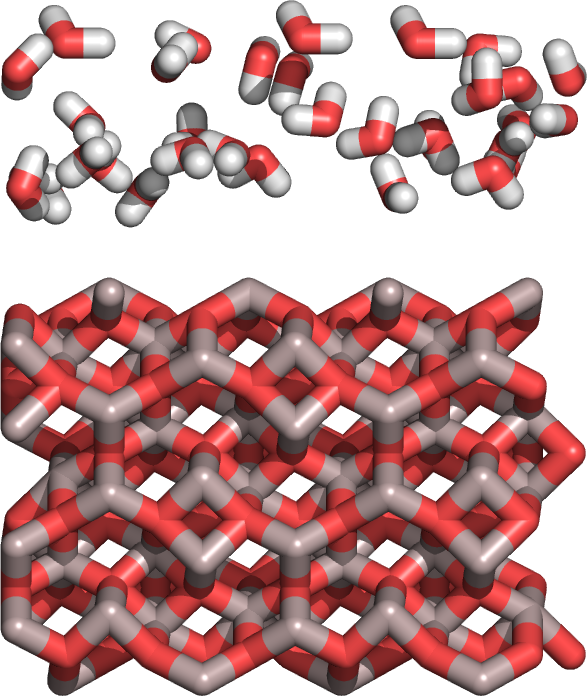
\includegraphics[width=\textwidth]{alumina_h2o_before}
    \subcaption{Seitenansicht, vorher}
    \label{fig:wateraluminasurface-a}
  \end{subfigure}
  \hfill
  \begin{subfigure}[t]{\subfigwidth}
    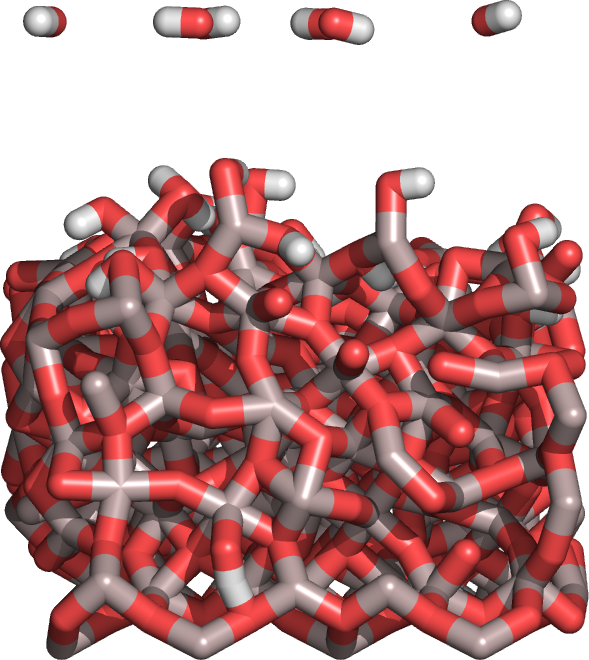
\includegraphics[width=\textwidth]{alumina_h2o_after}
    \subcaption{Seitenansicht, nachher}
    \label{fig:wateraluminasurface-b}
  \end{subfigure}
  \hfill
  \begin{subfigure}[t]{\subfigwidth}
    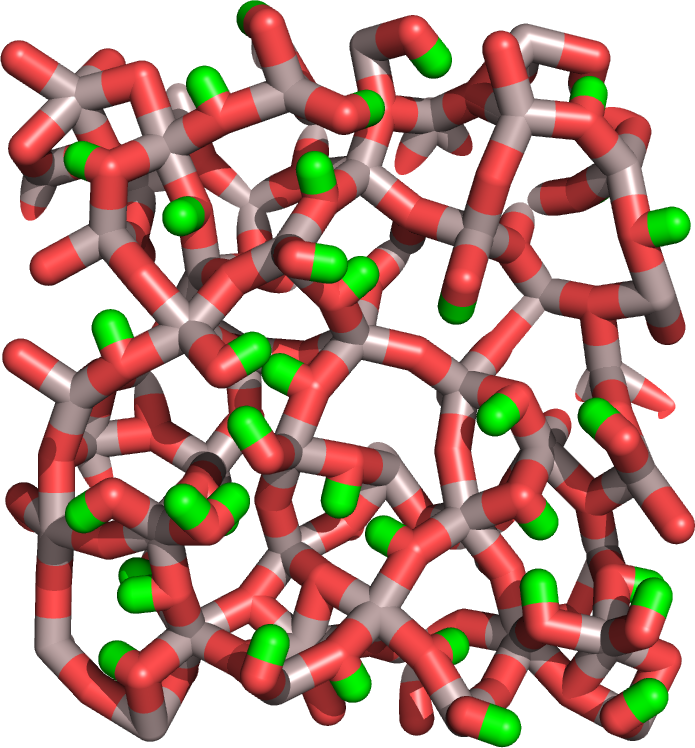
\includegraphics[width=\textwidth]{alumina_h2o_topview}
    \subcaption{Draufsicht, nachher.
      Hydroxyl ist grün hervorgehoben.
    }
    \label{fig:wateraluminasurface-c}
  \end{subfigure}
  \caption[Oberflächenreaktion von Wasser mit $\alpha$-\ce{Al2O3}]{Ergebnisse einer Oberflächenreaktion von Wasser mit $\alpha$-\ce{Al2O3}.
    Das Wasser reagiert mit Sauerstoffatomen an der Oberfläche zu Hydroxylgruppen.
  }
  \label{fig:wateraluminasurface}
\end{figure}

Das Ergebnis der Simulationen für die Liu-Parameter (Abbildungen \ref{fig:wateraluminasurface-c} und \ref{fig:wateraluminasurface-c}) zeigt die gleichmäßige Bedeckung der Oberfläche mit Hydroxylgruppen (\todo{tatsächlicher Wert!}\SI{19}{\per\square\nano\meter}) und gelegentlich adsorbierten Wassermolekülen.
Letztere sollten aber auf längere Sicht durch die Einflüsse der Überkoordinationsterme des ReaxFF-Potentiales entweder zerfallen oder sich von der Oberfläche lösen.
Trotz unterschiedlicher Startbedingungen stimmt der maximale Bedeckungsgrad der Oberfläche mit Hydroxylgruppen mit experimentell bestimmten Werten von \todo{eigentlicher Wert}\todo{Ref!}\SI{19}{\per\square\nano\meter} überein.
In diesen Startbedingungen wurde von einer ausreichenden Zahl von Wassermolekülen für \todo{tatsächliche Werte!}\SI{20}{\per\square\nano\meter}, \SI{50}{\per\square\nano\meter} und \SI{100}{\per\square\nano\meter} ausgegangen, von denen die überschüssigen Moleküle aber im Verlauf der Simulationen in der Gasphase verblieben sind, wie in Abbildung \ref{fig:wateraluminasurface-b} am oberen Rand der Simulationsbox erkennbar ist.

Mit den Narayanan-Parametern konnten diese Reaktionen aufgrund einer repulsiven Kraft zwischen den Wassermolekülen und der Oberfläche nicht simuliert werden.
Das deutet darauf hin, dass Hydroxylgruppen auf einer Aluminiumoxid-Oberfläche energetisch nicht bevorzugt werden oder der Übergang mit der Überwinding einer hohen Energiebarriere verbunden ist.

\subsection{Vollständige ALD-Simulationen}

\todo[inline]{continuehere}
